\documentclass{kthreport}
% default language is English, but you can use Swedish definitions like this:
% \documentclass[swedish]{kthreport}

% Remember that in order for the class to find the KTH logo, you need to
% have it in your path, for example:
% export TEXINPUTS=/path/to/logo/location//:$TEXINPUTS

\usepackage[libertine,cmintegrals,cmbraces,vvarbb]{newtxmath}
\usepackage[backend=biber, sorting=none]{biblatex}
\addbibresource{bibl.bib}
\usepackage{listings}
\usepackage{xcolor}
\usepackage[group-digits=true, binary-units=true]{siunitx}
\usepackage{caption}

\let\openbox\relax
\usepackage{amsthm}
\theoremstyle{definition}
\newtheorem{definition}{Definition}
\newtheorem{example}{Example}
\let\endopenbox\relax

\usepackage{amsmath}
\usepackage{csquotes}
\usepackage{enumitem}

\definecolor{dkgreen}{rgb}{0,0.6,0}
\definecolor{gray}{rgb}{0.5,0.5,0.5}
\definecolor{lightgray}{rgb}{0.95, 0.95, 0.95}
\definecolor{mauve}{rgb}{0.58,0,0.82}
\definecolor{mygreen}{rgb}{0,0.6,0}
\definecolor{mygray}{rgb}{0.5,0.5,0.5}
\definecolor{mymauve}{rgb}{0.58,0,0.82}
\lstdefinestyle{MyPython}{
	language=Python,
	frame=Lbtr,
	xleftmargin=\parindent,
	captionpos=b,
	aboveskip=3mm,
	belowskip=3mm,
	showstringspaces=false,
	columns=flexible,
	basicstyle={\small\ttfamily},
	numbers=left,
	numberstyle=\tiny\color{gray},
	keywordstyle=\color{purple},
	commentstyle=\color{gray},
	stringstyle=\color{dkgreen},
	breaklines=true,
	breakatwhitespace=true,
	tabsize=4,
	morekeywords={traci, print},
	otherkeywords={},
	backgroundcolor=\color{lightgray},
	escapeinside={/l*}{*l/}
}

\usepackage{url}

\newcommand{\suchthat}{\, \mid \,} % nice "such that"
\renewcommand{\thefootnote}{\fnsymbol{footnote}}
\newcommand{\twodots}{\mathinner {\ldotp \ldotp}}

%\DeclareFontFamily{\encodingdefault}{\ttdefault}{\hyphenchar\font=`\-}

\title{Final Assignment}
\subtitle{DD3431 Machine Learning (PhD variant)}
\author{Manuel Osvaldo Olguín}
\diarienr{01}

\begin{document}
\maketitle

This final report for the DD3431 Machine Learning course describes the application of Linear Support Vector Machines to a multi-class, multi-output classification problem modeling the resource allocation strategies for basestations in a 5G environment. The classifier was adapted to the multi-class nature of the output.

\section{Theoretical description of the problem}

\subsection{Description of the data}\label{sec:data}

The data used for this study corresponds to samples of the resource allocation strategy for a communication system composed of exactly three basestations and up to a maximum of \num{20} user devices. The area of interest studied within this communication scenario is modeled as a map; more specifically, it represents an area of \SI{2400}{\metre\squared} divided into a grid of \SI{2}{\metre}$\times$\SI{2}{\metre} cells. This grid is encoded as a matrix, with values between \num{0} and \num{2} indicating the occupancy status of each cell:
\begin{itemize}
	\item \num{0} for empty cells,
	\item \num{1} for cells occupied by a user device,
	\item \num{2} for cells occupied by a basestation.
\end{itemize}

The occupancy data for each user can either be perfect or have an inaccuracy defined by a normal distribution with three possible standard deviations: \num{0.1}, \num{0.25} or \num{0.4}. Thus, the model had to be trained a total of four times, one for each variation of the positioning inaccuracy -- we will call them \emph{scenarios}. The input data for each scenario corresponds then to the vectorized form of the corresponding matrix, i.e. a vector of \num{600}\footnote{$\frac{2400}{(2\times2)} = 600$} elements, each with a value $v_i \in \{0, 1, 2\}$.

On the other hand, the output data for the learning algorithm corresponds to encoded variables (\emph{labels}) representing the basestation--user device association and the resource allocation information for each sample. The exact details of this encoding and the information carried within escape the scope of this report, but it is of importance to note that:
\begin{enumerate}
	\item there are \num{9} of these output variables per input sample (\num{3} for each basestation in the model);
	\item these output variables are mutually independent;
	\item they have discrete integer values that range between \num{0} and \num{12288};
	\item the order in which these values appear in the output is relevant (i.e. permutations of the same values correspond to different interpretations of the output);\label{item:order}
    \item finally, these values can also be repeated across variables in the same output vector.\label{item:repeat}
\end{enumerate} 

Items \ref{item:order} and \ref{item:repeat} make the problem different than a ``regular'' multi-label classification problem, in which only the distinct \emph{sets} of labels matter \autocite{tsoumakas2006multi}. 
Item \ref{item:repeat} is in practice a consequence of \ref{item:order} -- the significance of the positions of the labels in the output means that repeated values don't have the same meaning since their positions in the output vector are different.
Additional preprocessing was thus necessary to adapt the output to traditional multi-label classification methods; this is discussed in section \ref{sec:cfchoice}.

In summary, the structure of an arbitrary sample looks like the following:

\begin{equation}
\underbrace{0, 1, 0, 0, 2, 0, \ldots 0, 0, 0, 0, 0, 1,}_{\text{600 input features}}\underbrace{4567, 23, \ldots , 1337}_{\text{9 output labels}}
\end{equation}

In total, \num{72000} samples in this format for each scenario were provided for the training of the model, with two thirds (\num{48000}) of these used for fitting and the rest (\num{24000}) used for validation purposes. The complete dataset was also used for \num{10}-fold cross-validation, again for each scenario.

%\subsection{Adapting the data} \label{sec:problemtransform}

% As described in the previous section, the data represents a multi-class, multi-label problem with a high dimensionality both in terms of input features and classes, with the additional restriction that the order of the output labels matters. %\autocite{tsoumakas2009mining}.

\subsection{Choice and adaptation of classifier}\label{sec:cfchoice}

The dataset in question is part of ongoing research at the Department of Information Science and Engineering of the School of Electrical Engineering, and has already been modeled with great success using Random Forests and Neural Networks. The application of Support Vector Machines was then a natural step given this models' popularity in networking research literature; the specific application of the Linear Kernel for SVMs was a result of exploratory analysis with the dataset in the early stages of development, where initial experiments exposed the linearly separatable nature of the output variables.

Support Vector Machines are binary classifiers though, and thus additional modifications are required to adapt these classifiers to multiclass problems as the one in question. Specifically, the following techniques for adapting binary classifiers to multiclass applications were identified from literature \autocite{hsu2002comparison,tax2002multiclass}:

\begin{description}
	\item[One-vs-One Method:] For a universe $K$ of classes, with $\kappa = |K|$, this method constructs a maximum of $(\kappa(\kappa-1)/2)$ classifiers\footnote{This number could be smaller, as only the classes actually present in the training data are used.}, each comparing a pair of classes from the training set. For prediction, all of these classifiers are applied to an unseen sample, whose final class corresponds to the class with the most ``votes'' after processing. In case of a tie, it selects the class with the highest total confidence, obtained by aggregating the confidence scores of each binary classifier.
	\item[One-vs-Rest Method:] Constructs a maximum of $\kappa$ classifiers, each comparing one class in the training set with the rest (i.e. each classifier determines if a sample belongs to a specific class or not). At prediction time, these classifiers are applied to the unseen sample and it is once again classified according to the majority vote.
\end{description}

Other multiclass adaptations of binary classifiers, like DAGSVM \autocite{chen2009dagsvm} and DDAG \autocite{platt2000ddag} were considered as well, but were ultimately judged to be overly complex for the problem at hand.

Note though that all of these modifications only transform a binary-class single-label classifier into a multi-classs single-label classifier, \emph{i.e.} they don't adapt the classifier to output more than one output variable (label) per prediction.
Thus, another modification to the problem was necessary, as changing the classifier was discarded from the beginning.

Two problem transformation strategies were evaluated: the \emph{Binary Relevance} and the \emph{Label Powerset} transformations \autocite{tsoumakas2006multi}:

\begin{description}
    \item[Binary Relevance:] This problem transformation learns $\kappa = |K|$ binary classifiers -- where $K$ again is the universe of classes, \emph{i.e.} one binary classifier for each class. Then, for an unseen sample $i$, it applies all $\kappa$ classifiers to it and assigns to it the union of all labels returned.
    \item[Label Powerset:] This transformation is based on treating each distinct set of labels in the training output as a separate \emph{meta-label}. It thus trains \emph{one} multi-class classifier on $\eta$ input samples with $|\Lambda|$ possible output meta-labels, where $\Lambda$ is the collection of unique label combinations present in the original training output. 
    Since it basically converts the problem into a single multi-class classification scenario, this strategy only works well if the number of samples is much larger than $|\Lambda|$.
\end{description}

The final decision about which multi-class classifier and problem transformation to use was mostly based on time efficiency. The large dimensions of the problem meant that less time-efficient classification methods could take extremely long times to fit and validate, without proportional gains in accuracy. Thus, the in the end the following methods were selected for the assignment:

\begin{description}
    \item[Multi-class classifier:] The \emph{One-vs-Rest} method was selected to adapt Support Vector Machines to the multi-class problem at hand, specifically because it only needs to train $\kappa$ classifiers instead of $\kappa(\kappa-1)/2$ (this number could be very big).
    \item[Problem transformation:] It quickly became evident in the early exploratory stages of this assignment that the binary relevance method would be very unpractical. Given the large universe of labels of the problem ($ K = [0 \twodots \num{12288}] \Rightarrow |K| = \num{12289}$) and the large number of samples available, this method would take large amounts of time to both fit and validate.
    
    On the other hand, exploratory analysis of the input data revealed there were only about \num{800} distinct output label permutations in the \num{48000} training samples for each scenario, which meant that the Label Powerset method was applicable to this problem. 
\end{description}

This combination of methods meant that only \emph{one} multi-class Support Vector Machine, comprised of about \num{800} binary SVMs (one for each \emph{meta-label} versus the rest), needed to be trained for each scenario. In contrast, the number of of classifiers that need to be trained for each of the other combinations is:

\begin{itemize}
    \item For the binary relevance transformation using binary SVM's (since this method works directly with binary classifiers), \num{12289} classifiers need to be trained for each scenario.
    \item For \emph{One-vs-One} multi-class SVM's using the Label Powerset transformation, approximately $800(800-1)/2 = \num{319600}$ classifiers need to be trained. 
\end{itemize}

Traditional multi-label classification methods don't take into consideration the positions or the repetition of output labels though -- only the distinct \emph{sets} of output labels are considered relevant \autocite{tsoumakas2006multi}. Thus the problem had to be transformed in such a way that the positional information of each label in the output was encoded into the \emph{meta-label} used by the Label Powerset transformation.

The following transformation $F_{\text{enc}}$ was used then to adapt the training data:

\begin{definition}
     Given a label output vector $\vec{\Omega} = [\vec{\nu_{0} \dots \nu_{9}}]$, with $\nu_{i} \in K$, $i \in [0 \twodots 9]$:
    
    \begin{equation}\label{ec:fenc}
    F_{\text{enc}}:\ \vec{\Omega} \rightarrow \Omega' \quad \left\vert \quad
    \begin{aligned}
    \Omega' &= \{\nu'_{0}, \ldots, \nu'_{9}\} \\
    \nu'_{i} &= i|K| + \nu_{i} \qquad i \in [0, 9]
    \end{aligned}\right.\\
    \end{equation}
\end{definition}


%Where $\nu$ is the value of the output variable (label), $i$ corresponds to the $0$-indexed position of the variable in the output vector and $K$ is the universe of valid labels ($K = [0, 12288]$ in this particular case). 
In practice, the result of this transformation is that the range of each output label in the original sample is modified so that it is distinct from the output range of every other label in the same sample. 
The first label retains its range (between \num{0} and $|K| - 1$), whereas the second label has its range shifted to $[|K|\twodots2|K| - 1]$, the third label to $[2|K|\twodots3|K| - 1]$ and so on.
Thus, the new label set $\Omega'$ has no repeated values, and although in the definition of $F_{\text{enc}}$ the new labels maintain their respective positions from $\vec{\Omega}$, this is ultimately irrelevant as all positional information is encoded in the new values $\nu_{i}'$. 
This last detail is specially relevant when obtaining prediction results from the classifier since, as we will explain in section \ref{sec:parsing}, multi-label classifiers only return \emph{sets} of labels associated with a sample, without any information about the labels relative positions in the output.

Finally, to revert $F_{\text{enc}}$ and obtain $\vec{\Omega}$ from $\Omega'$, for instance when using the classifier for predictions, one only needs to apply the following transformation:

\begin{definition} Given a label \emph{set} $\Omega'$,
    \begin{equation}
    F_{\text{dec}}:\ \Omega' \rightarrow \vec{\Omega} \quad \left\vert \quad
    \begin{aligned}
    \vec{\Omega} &= [\vec{\nu_{0}, \ldots, \nu_{9}}] \\
    \nu_{i} &= \left \{
    \begin{aligned}
    \nu &= \nu' \bmod |K| \qquad \nu' \in \Omega'\\
    i &= \frac{\nu' - \nu}{|K|}
    \end{aligned}\right.\\
    \end{aligned}\right.\\
    \end{equation}
\end{definition}


\section{Implementation}

\subsection{Language and libraries used}

The language chosen for this project was Python 3.6, given its extensive support for scientific programming, data analysis and machine learning in the form of libraries. In particular, the libraries \textbf{scikit-learn} (and its multilabel extension, \textbf{scikit-multilearn}), \textbf{scipy}, \textbf{matplotlib} and \textbf{numpy} were used for the implementation \autocite{scikit-learn,scikit-multilearn,scipy,matplotlib,numpy}.

\subsection{Choice of classifier}

Based on the analysis detailed in section \ref{sec:cfchoice}, \textbf{sklearn.svm.LinearSVC} was selected as the base classifier to be used for this problem, as it corresponds to an implementation of a multi-class Support Vector Machine using the \emph{One-vs-Rest} method and a linear kernel. Tests were also conducted with \textbf{sklearn.svm.SVC}, which implements a multi-class SVM using the \emph{One-vs-One} method and a RBF-kernel, but its runtime proved to be cumbersomely large\footnote{Not a fair comparison, but for the unoptimized SVC case the runtime was over \num{3} hours for fitting and predicting, whereas the final runtime for the optimized and parallelized LinearSVC is, on average, \num{110} seconds.}.

The classifier was then extended to work on multilabel outputs through the \textbf{skmultilearn.problem\_transform.LabelPowerSet} class, which implements the \emph{Label Powerset} problem transformation as detailed in \ref{sec:cfchoice}. 
Thus, the classifier treats every distinct label combination in the training data as a separate class or \emph{meta-label} when fitting and predicting.

\subsection{Parsing and adapting the data}\label{sec:parsing}

The data provided for building the model consisted of \num{72000} samples for each of the four positional accuracy values detailed in the problem description (section \ref{sec:data}), divided into two files each: \num{48000} of the samples for training, and \num{24 000} for validation. The format of the input files was one sample per line: \num{600} integers with values in $\{0, 1, 2\}$ representing the input features, followed by \num{9} integers with values in $[0 \twodots 12288]$ representing the output variables (everything separated by commas, see example in listing \ref{lst:example1}).

\begin{figure*}[tb]
\begin{lstlisting}[captionpos=b,
basicstyle={\small\ttfamily},
numbers=left, 
numberstyle=\tiny\color{gray},
caption={Abbreviated example of input samples.},
label={lst:example1}]
0,0,0,...,0,2,0,...,3968,3841,528,8080,4209,6273,9201,9073,8592
0,0,0,...,0,2,0,...,80,2545,2417,6145,8176,4112,8443,11761,8736
0,0,0,...,0,2,0,...,3680,0,0,4112,8017,7408,10241,8272,11505
\end{lstlisting}
\end{figure*}


This data was parsed using \textbf{numpy}'s \textbf{loadfromtxt()} function, and then split into separate arrays for the input and output data (labels). The input data was passed ``as-is'' to the classifier, but the output data required additional processing which will be detailed below.


As mentioned before, the output labels for each case were presented in the form of \num{9} consecutive integers, each ranging in value from \num{0} to \num{12288}. On the other hand, as per the API specifications\footnote{\url{http://scikit.ml/api/datasets.html#the-multi-label-data-representation}} of \textbf{scikit-multilearn}, when using the \textbf{LabelPowerSet} problem transformation, the output labels passed to (and obtained from) the classifier need to be encoded into a \emph{binary indicator matrix}. 

\begin{definition}
	A binary indicator matrix for a set of $\eta$ samples, with a universe $K$ of output labels, is a matrix $A$ of dimensions $(\eta \times |K|)$, where
    
    \begin{align}
        A &= 
        \begin{bmatrix}
        a_{0,0} & \cdots & a_{0, \kappa}\\
        \vdots & \ddots & \vdots \\
        a_{\eta, 0} & \cdots & a_{\eta, \kappa}
        \end{bmatrix}
        \qquad \kappa = |K|\\
    	(a_{i,j}) &= \begin{cases}
        	1\ \text{if label}\ j \in K\ \text{is assigned to sample}\ i \\
        	0\ \text{otherwise}
    	\end{cases}
    \end{align}
	
	Thus, $A$ is a sparse matrix where each row has \emph{at most} $\gamma$ elements of value $1$, where $\gamma$ is the number of output labels associated with each sample.
\end{definition}

Note that binary indicator matrices \emph{do not preserve information about label positions} in the output.
Consider two sets of labels $\alpha$ and $\beta$, where $\beta$ is a permutation of $\alpha$ -- i.e. both have the same labels but in different order. 
Given the previous definition of a the binary indicator matrix, both sets would then have the same representation in the matrix, since each element of a row only indicates if the label is present in the output. 
They also don't handle repeated labels correctly -- multiples of a label are all assigned to the same element of the matrix. This is directly related to the fact that multi-label classification problems are defined as classification problems in which the output is a label \emph{set}, as opposed to a label \emph{vector} \autocite{tsoumakas2006multi}. Each row of the binary indicator matrix can thus be seen as the matrix representation of the elements present in a specific set.

The preprocessing of the training data label output vectors using $F_{\text{enc}}$ (see equation \ref{ec:fenc}) solves these problems, as explained in section \ref{sec:cfchoice}. The new values obtained with $F_{\text{enc}}$ do not overlap with each other -- solving the repetition problem -- and encode the positional data of each label in the original output vector together with the actual value of said label. 
These new values can then be encoded into a binary indicator matrix without any loss of information by simply extending their range to be the aggregate of the ranges of each of them. 
For instance, for $\gamma$ output variables, their common range $|K'|$ can be interpreted as being $\gamma \times |K|$, and thus they can be encoded into a binary indicator matrix of dimensions $(\eta \times \gamma|K|)$ where the first label occupies the first $|K|$ places of each row, the second label places between $|K|$ and $2|K|$ and so on.
 
In the same vein, prediction values obtained from the classifier have these same properties (since the classifier was trained on them), and can be decoded into output vectors using $F_{\text{dec}}$.

\begin{figure*}[tb]
	\begin{lstlisting}[style=MyPython, caption={Encoding function in Python. This function both transforms the given output label matrix using $F_{\text{enc}}$ and encodes the result into a binary indicator matrix.}]
def encode_output(output):
	"""
	Processes the given label set output matrix to the binary representation
	expected by scikit-multilearn
	:param output: Label set output matrix
	:return: Binary representation of input matrix
	"""
	processed_output = dok_matrix((len(output), 
							n_labels * n_classes), 
							dtype=np.uint8)
	
	for i, row in enumerate(output):
		for j, label in enumerate(row):
			processed_output[i, (j * n_classes) + label] = 1
	
	return processed_output.tocsr()
		\end{lstlisting}
\end{figure*}

\begin{figure*}[tb]
	\begin{lstlisting}[style=MyPython, caption={Decoding function in Python, which takes a binary indicator matrix and extracts and decodes the encoded values within using $F_{\text{dec}}$.}, label={lst:decode}]
def decode_output(encoded_output):
	"""
	Decodes a binary indicator matrix into a 2-D vector 
	of label vectors. Each row in the output corresponds 
	to the label vector for a specific sample.
	:param encoded_output: Binary indicator matrix.
	:return: 2-D vector of label vectors.
	"""
	n_zero = encoded_output.nonzero()
	decoded_output = np.empty(shape=(encoded_output.shape[0],
							n_labels),
							dtype=np.uint16)
	for row, col in zip(*n_zero):
		value = col % n_classes
		decoded_col = int(col - value) / n_classes
		decoded_output[int(row), int(decoded_col)] = value
	
	return decoded_output
	\end{lstlisting}
\end{figure*}

\subsection{Fitting and validating the model}

Fitting and predicting on the test datasets and validating the results were performed in parallel for the four scenarios using a Python process pool (\textbf{multiprocessing.Pool}). 

For each scenario, a classifier was constructed using the \textbf{LabelPowerSet} class with a \textbf{LinearSVC} using default parameters as the base classifier, which was then fitted on the training input data and the associated binary indicator matrix for the processed label output data using the \textbf{fit()} method of the classifier.
Next, the model was validated on the training data using a custom accuracy score function which takes advantage of the matrix representation of the results and of the fact that the position of each label matters in the final result. 

\begin{definition}
    Let $V$ be the binary indicator matrix for the labels for the test fraction of the dataset (\emph{i.e.} the expected output), and $V'$ the output generated by the classifier for the test input data, then the accuracy score function $f_{acc}$ can be expressed as:
    
    \begin{equation}\label{ec:acc}
    f_{acc}(V, V') = 1 - \frac{\text{nonzero}(V - V')}{2 \times \text{nonzero}(V)}
    \end{equation}
\end{definition}

In words, equation \ref{ec:acc} first calculates the total number of non-zero elements in the element-by-element difference between both matrices; since both matrices have exactly the same amount of non-zero elements per row (by definition, thanks to the previously discussed encoding function), this amount will actually be double the real amount of discrepancies (since each ``error'' will appear twice in the difference matrix, once for the value in the validation matrix and once for the value in the output matrix).
This value is then divided by two to get the correct amount of errors, before being divided by the total expected number of output values in the validation matrix to get the decimal representation of the error in the classification.
Finally, this value is subtracted from $1$ to get the total accuracy value of the model for the given training data. 

\begin{figure*}[tb]
\begin{lstlisting}[style=MyPython, caption={Accuracy score function implemented in Python}]
def accuracy_score(x1, x2):
    assert x1.shape == x2.shape
    assert x1.nnz == x2.nnz
    errors = (x1 - x2).nnz / 2.0
    return 1.0 - (errors / x1.nnz)
\end{lstlisting}
\end{figure*}

After validation of the results, the accuracy score values are printed to standard output for review. 
The predictions generated by the classifier for each scenario are ``decoded'' (using $F_{\text{dec}}$ as detailed in listing \ref{lst:decode}) back the to dataset format for output labels (i.e, vectors of nine integers between \num{0} and \num{12288} each) and written to CSV-formatted text files for future use.

\subsection{k-fold cross-validation}

Although \textbf{scikit-learn} includes a function for k-fold cross-validation, it quickly became evident that an adapted, more optimized implementation was required. 
In particular, the built-in function uses the default accuracy score function, which doesn't take into account the position of the labels in the final output vector. The library's cross-validation function is also not parallelized, which greatly hampers its runtime.

A new, custom, k-fold cross-validation was then implemented taking these caveats into consideration; it first shuffles the input data and then proceeds to execute the folds in parallel on four concurrent processes. See listing \ref{lst:kfoldcv} for details.


\section{Results and brief conclusion}

The results obtained were highly encouraging.
Table \ref{tbl:accuracy} exposes the accuracy scores obtained for the classification tasks, \emph{i.e.} fitting the linear multi-class support vector machines on the \num{48000} training samples available for each scenario and then validating on the respective \num{24000} samples available for each. 
The results for the \num{10}-fold cross-validation tasks are also presented, in table \ref{tbl:10foldcv}.

Performance metrics for the fitting, validating and cross-validating of the data were also evaluated for future reference; specifically, we recollected information on the runtime of each stage along with the CPU and RAM usage of the program. 
The specifications of the system on which the experiments were performed can be found in table \ref{tbl:specs}, whereas the results of these measurements can be studied in table \ref{tbl:runtime} and figures \ref{fig:cpu} and \ref{fig:ram}.

To conclude, these scores demonstrate not only the applicability of Support Vector Machines to the problem, but also their efficacy and great accuracy. Even though the challenge tackled in this assignment corresponds to a multi-class, multi-label problem, a group of problems for which SVM's are rarely considered, accuracy scores over \SI{91}{\percent} for all the scenarios show that SVM's can in fact be a powerful tool for this category of problems.

\begin{table}[tb]
    \centering
    \begin{tabular}{|l|l|}
        \hline
        Processor & Intel Core i7-\num{6700} (4 cores/8 threads) @ \SI{4}{\GHz})\\
        Memory & \SI{32}{\gibi\byte} DDR4\\
        OS & Ubuntu 17.10\\
        \hline
    \end{tabular}
    \caption{System specifications.}
    \label{tbl:specs}
\end{table}

\begin{figure*}[tb]
        \centering
        \begin{tabular}{|l|c|}
            \hline 
            \textbf{Scenario} & \textbf{Accuracy Score} \\ 
            Perfect position information & \num{0.9926} \\ 
            Position with gaussian error - std = \num{0.10} & \num{0.9858} \\ 
            Position with gaussian error - std = \num{0.25} & \num{0.9556} \\ 
            Position with gaussian error - std = \num{0.40} & \num{0.9177} \\ 
            \hline 
        \end{tabular}
        \captionof{table}{Accuracy results for each scenario on the respective test datasets.}
        \label{tbl:accuracy}%
        \bigskip%
        \begin{tabular}{|l|c|c|}
            \hline 
            \textbf{Scenario} & \textbf{Avg. Accuracy} & \textbf{STD} \\ 
            Perfect position information & \num{0.9982} & \num{0.0003} \\ 
            Position with gaussian error - std = \num{0.10} & \num{0.9985} & \num{0.0002} \\ 
            Position with gaussian error - std = \num{0.25} & \num{0.9985} & \num{0.0002} \\ 
            Position with gaussian error - std = \num{0.40} & \num{0.9994} & \num{0.0003} \\ 
            \hline 
        \end{tabular}
        \captionof{table}{Results for the \num{10}-fold cross-validation tasks.}
        \label{tbl:10foldcv}%
        \bigskip%
        \begin{tabular}{|l|c|}
            \hline
            \textbf{Task} & \textbf{Avg. Time [s]}\\ 
            Fit Classifier & \num{107.78} \\ 
            Validate on test data & \num{2.04} \\ 
            10-fold cross-validation & \num{489.93} \\ 
            \hline 
        \end{tabular} 
        \captionof{table}{Average runtime for each stage of the program.}
        \label{tbl:runtime}
\end{figure*}

\subsection{Sources}

The source code and data for this assignment can be found on the authors' personal GitHub repository: \url{https://github.com/molguin92/KTH_MachineLearning}.

\newpage
\printbibliography%[heading=none]
\newpage
\begin{lstlisting}[style=MyPython, caption={Extract of the k-fold cross-validation subroutines.}, label={lst:kfoldcv}]
def cross_validation_fold(index, splits_in, splits_out):
	"""
	k-fold cross-validation "fold": performs validation using 
    exactly one of the splits as validation set and the rest 
    of the dataset as training data.
	:param index: Index of the split to use as validation data
	:param splits_in: List of splits of the original 
        dataset inputs
	:param splits_out: List of splits of the original 
        dataset outputs
	:return: The accuracy score for a LinearSVC trained on 
        all the splits except <index> and then validated 
        on split <index>
	"""
	validation_in = splits_in[index]
	validation_out = splits_out[index]
	cf = LabelPowerset(LinearSVC())
	
	# train on all splits except split <index>
	cf.fit(np.vstack(splits_in[:index] + splits_in[index + 1:]),
		sparse_vstack(splits_out[:index] + splits_out[index + 1:]))
	
	# validate on split <index>
	return validate(cf, validation_in, 
                    validation_out, 
                    return_predictions=False)

def k_fold_cross_validation(dataset, k=10):
	"""
	Performs k_fold cross validation on a dataset using LinearSVCs
	:param dataset: Dataset tuple in format 
    (train_in, train_out, test_in,test_out)
	:param k: Optional k-fold parameter. Default is 10.
	:return: Tuple containing the average accuracy and 
        standard deviation obtained through 
        cross-validation.
	"""
	
	assert k > 1
	
	# label data has to be dense to be shuffled
	# in the same order as the input data
	data_in = np.vstack((dataset[0], dataset[2]))
	data_out = np.vstack((dataset[1].toarray(),
                        dataset[3].toarray()))
	
	# shuffle data, then partition
	data_in, data_out = shuffle_data(data_in, data_out)
	data_in = np.split(data_in, k)
	data_out = np.split(data_out, k)
	
	# re-sparsify?
	data_out = list(map(csr_matrix, data_out))
	
	results = None
	with Pool(processes=4) as pool:
		results = pool.starmap(cross_validation_fold,
                                zip(range(k),
                                    itertools.repeat(data_in),
                                    itertools.repeat(data_out)))
	
	results = np.array(results)
	return results.mean(), results.std()
\end{lstlisting}

\begin{figure}[p]
    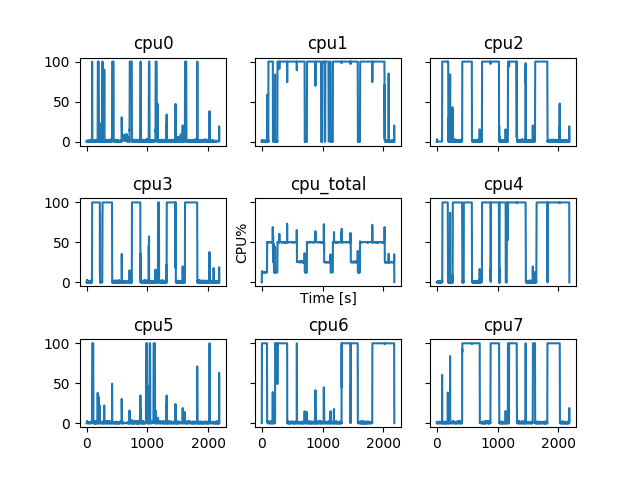
\includegraphics[width=\linewidth]{cpu.png}
    \caption{CPU usage for each logical core, along with the total aggregated CPU usage, over time.}
    \label{fig:cpu}
\end{figure}

\begin{figure}[p]
    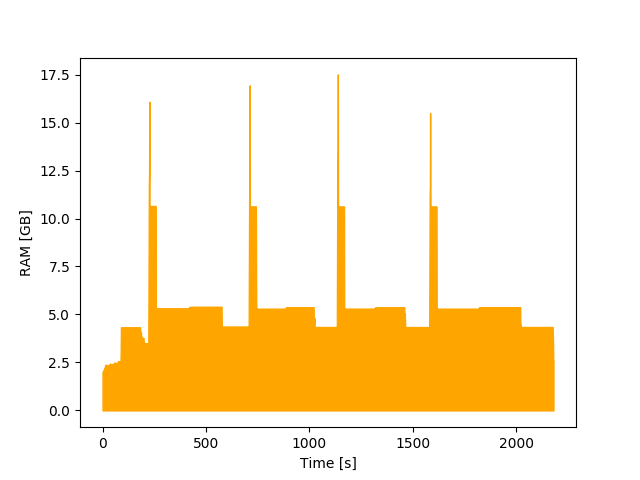
\includegraphics[width=\linewidth]{ram.png}
    \caption{RAM usage during execution of the program.}
    \label{fig:ram}
\end{figure}

\end{document}
